\documentclass{beamer}

\usepackage{wrapfig}
\usepackage{algpseudocode}
\usepackage{algorithm}
\usepackage[english]{babel}
\usepackage[sortcites,style=numeric,sorting=none,backend=biber]{biblatex}
\usepackage[export]{adjustbox}
\usepackage{eurosym}

\usetheme{Boadilla}
\usecolortheme{dolphin}

\setbeamertemplate{navigation symbols}{}
\setbeamertemplate{sections/subsections in toc}[sections numbered]

\setbeameroption{hide notes}

\addbibresource{ref.bib} %Imports bibliography file
% \setbeameroption{show only notes}
% \setbeameroption{show notes on second screen=right}

\title[Tracing Features in ARM]{Tracing Features in ARM Embedded Systems:}
\subtitle{Exploring Ideas and Leveraging Existing Capabilities for Enhanced
Trace Capturing Performance via A Cost Efficient Hardware}
\author[]{Hossein Afkar}
\institute{DRTS Lab}
\date{\today}

\begin{document}

\frame{\titlepage}

\begin{frame}
    \frametitle{Outline}
    \tableofcontents[hideallsubsections]
\end{frame}

\AtBeginSection[]
{
    \begin{frame}{Outline}
        \tableofcontents[currentsection]
    \end{frame}
}


\section{Introduction}
\begin{frame}
    \frametitle{Preface}
    \begin{itemize}
        \item Trace: A detailed record of how software is
            executed by an SoC's processor.
        \item Tracing plays a crucial role in understanding the
            behavior and performance of embedded systems.
        \item We will cover the general features of the Embedded Trace
            Macrocell (ETM) and its extensive trace capabilities.
        \item Existing trace hardware options, including their cost and
            performance considerations, will be examined.
        \item Existing ideas related to tracing will be explored.
    \end{itemize}
\end{frame}

\section{Embedded Trace Macrocell}
\subsection{General ETM Features}
\begin{frame}
    \frametitle{Embedded Trace Macrocell}
    Embedded Trace Macrocell (ETM) is a real-time trace module providing
    instruction and data tracing of a processor.
    \begin{itemize}
        \item Features extensive instruction and data tracing capabilities.
        \item Provides an extensible specification for controlling the trace
            via triggers and filtering resources.
    \end{itemize}
\end{frame}

\begin{frame}
    \frametitle{Tracing Triggers}
    Events control the Trace Enable Signals without any other interferences.
    \begin{itemize}
        \item Data and Instrunctions Address Comparators.
        \item Context ID Comparators. (Dependent on the OS)
        \item Virtual Machine ID Comparator.
        \item Memory Map Decoders.
        \item EmbeddedICE Module Watchpoint Comparators.
        \item Counters.
        \item Three-state Sequencer.
        \item External Inputs (Imprecise).
        \item Software Instrumentation (Imprecise).
    \end{itemize}
\end{frame}

\begin{frame}
    \frametitle{Imprecise Trace Generation}
    Tracing can be imprecise. If the trace is imprecise
    following issues might happen:
    \begin{itemize}
        \item Tracing may not be turned on or off in time.
        \item data for an instruction might not be traced.
    \end{itemize}
    Tracing can be imprecise because of following events:
    \begin{itemize}
        \item Address Comparator configured for Fetch-stage instruction.
        \item Address Comparator with its exact bit set to 1
            (ETMv2.0 and later).
        \item Address Comparator configured for data addresses
            (before ETM v1.2).
        \item Address Comparator connected with Context ID comparator.
        \item A memory map decoder.
    \end{itemize}
    Some events are implementation defined. it is best to consult the
    documentation for our specific chip. \cite{arm2020embedded}
\end{frame}

\subsection{Timing Capabilites}
\begin{frame}
    \frametitle{Cycle Accuracy}
        \begin{itemize}
        \item \textit{ETMCR} controls the behavior of the ETM macrocell.
        \item Cycle accuracy is done by setting the bit 12 of the \textit{ETMCR}.
        \item Timestamping also happens in ETM. There are various events that
            cause the ETM module to generate a timestamp packet in the trace
            (T-Sync Packet).
            \begin{itemize}
                \item Enables us to correlate between different trace streams.
                \item Simple analysis of code performance.
                \item Timestamps are generated in a periodic way.
                    It is controlled by \textit{ETMSYNCFR}.
            \end{itemize}
    \end{itemize}
\end{frame}

\begin{frame}
    \frametitle{Instruction Tracing Representation}
    \begin{itemize}
        \item Instruction Tracing is represented by:
            \begin{itemize}
                \item P-Header packets.
                \item Branch packets (Indirect branch).
                \item Context ID packets (Indicate change in memory map or
                    executing process).
            \end{itemize}
        \item Cycle Accuracy is enabled by \textit{ETMCR}.
            \begin{itemize}
                \item Represented in P-Header packets.
                    \begin{itemize}
                        \item E: Instruction is executed and condition code is
                            passed.
                        \item N: Failed condition test.
                        \item W: Cycle boundary.
                        \item Example: \textcolor{red}{W}E\textcolor{red}{W}E\textcolor{red}{W}N\textcolor{red}{W}EE, \textcolor{red}{WW}E\textcolor{red}{WWW}E.
                    \end{itemize}
                \item Cycle count is stored in 32 bit values.
                \item Overflowing in cycle count causes the trace to be
                    inaccurate.
            \end{itemize}
    \end{itemize}
\end{frame}

\subsection{Trace Collection and Required Hardwares}
\begin{frame}
    \frametitle{Collecting Trace}
    \begin{itemize}
        \item Collecting trace is almost non-invasive: \cite{arm2020embedded}
            \begin{itemize}
                \item Power is affected.
                \item Trace consumes bandwidth on the processors bus therefore
                    QoS is required in the systems interconnects.
                \item According to the Ning et al., (2017)\cite{ning2017ninja} less than 0.1\% of the
                    processors performance is affected
            \end{itemize}
        \item There are various trace sinks in an ARM system that support ETM:
            \begin{itemize}
                \item Embedded Trace Buffer (4 KiB on Cortex-M).
                \item Trace Port Interface Unit (1000 Mbps for 4-bit TPIU).
            \end{itemize}
        \item How much we need:
            \begin{itemize}
                \item For a 200Mhz Cortex-M4 and the ITM its nearly about 324Mbps.
            \end{itemize}
    \end{itemize}
\end{frame}

\begin{frame}
    \frametitle{Existing Trace Hardware}
    \begin{itemize}
        \item Existing Hardware:
            \begin{itemize}
                \item Expensive (TPIU):
                    \begin{itemize}
                        \item 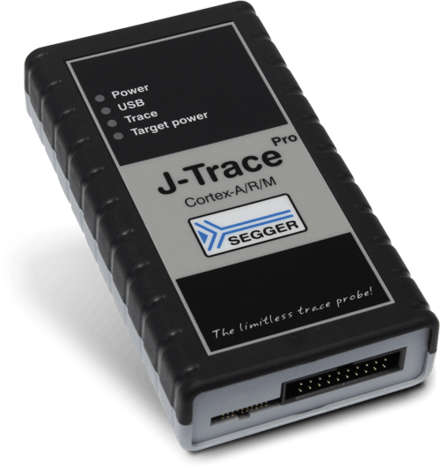
\includegraphics[width=1.3cm,valign=c]{jtraceARM.png} J-Trace Cortex-A/R/M, 1980\euro.
                        \item 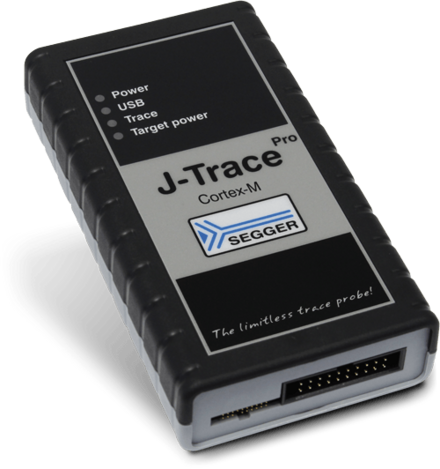
\includegraphics[width=1.3cm,valign=c]{jtraceM.png} J-Trace Cortex-M, 1490\euro.
                        \item 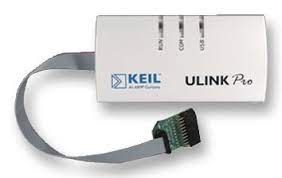
\includegraphics[width=1.3cm,valign=c]{ulink.jpeg} Keil ULINKpro (not ULINKpro D), 987\euro.
                    \end{itemize}
                \item Slow (SWO and JTAG):
                    \begin{itemize}
                        \item Any JTAG interface.
                        \item FT232RL (6.4 Mbps).
                    \end{itemize}
            \end{itemize}
    \end{itemize}
\end{frame}

\begin{frame}
    \frametitle{OrbTrace}
    A low cost, open source, Debug and Parallel Trace interface for
    CORTEX-M class embedded micro controllers.
    \begin{itemize}
        \item Support for 4-bit TPIU.
        \item Support for SWO at 62Mbps.
        \item USB 2.0 interface (480Mbps).
        \item Open-Source and Extensible.
        \item Rough BOM
            \begin{itemize}
                \item ECP5 FPGA LFE5U-25F 15\euro.
                \item 64 Mbit SDRAM 2W956A8MBYA5I 1.87\euro.
                \item USB3343-CP USB Driver Interface 1.61\euro.
                \item 8x Bus Transceiver SN74AVC2T245RSWR 0.99\euro.
                \item Rough Sum without connectors and parts costing less
                    than 1\euro: 26.4\euro + Roughly 10\euro for PCB manufacturing.
            \end{itemize}
    \end{itemize}
\end{frame}

\section{Exploring Ideas}
\subsection{Tracing for Monitoring Purposes}
\begin{frame}
    \frametitle{HART: Hardware Assisted Kernel Module Tracing in ARM}
    \begin{itemize}
        \item Used ETM with ETB to generate trace. Du et al.\cite{du2020hart}
        \item The goal is to provide an interface for users to build further
            monitoring capabitlites for kernel modules.
        \item Made HASAN as an interface to implement address sanitaion.
            \begin{itemize}
                \item Use after free (dangling pointer dereference)
                \item Heap buffer overflow
                \item Stack buffer overflow
                \item Global buffer overflow
                \item Use after return
                \item Use after scope
                \item Initialization order bugs
                \item Memory leaks
            \end{itemize}
        \item Incurs 6\% to 5\% of overhead.
        \item KASAN-enabled kernel incurs 4x slowdown in overall.
        \item Generate an interrupt using PMCs in order to avoid Overflowing in
            ETB buffer.
    \end{itemize}
\end{frame}

\subsection{Cycle Accurate Tracing}
\begin{frame}
    \frametitle{FrankenTrace}
    FrankenTrace a tool for non-invasive cycle-level PC and
    trace and LSU trace of some level of invasiveness. Matraszek et al.\cite{matraszek2023frankentrace}
    \begin{itemize}
        \item Only use low speed components that are present in cheap
            MCUs (DWT, ITM, SWO) and use cheap logic
            analyzers and serial monitors (FT232RL).
        \item Calls itself accurate cycle-level PC trace using
            low-speed debugging hardware.
        \item Calls ETM unreliable due to buffer overflows.
        \item Their method is based on repeatability.
            Requires each run to be identical.
    \end{itemize}
\end{frame}

\subsection{Tracing For Fuzz Testing}
\begin{frame}
    \frametitle{$\mu$AFL: Non-intrusive Feedback-driven Fuzzing
    for Microcontroller Firmware}
    \begin{itemize}
        \item $\mu$AFL is a new fuzzing tool designed for MCU firmware fuzzing,
            with a focus on peripheral driver code. \cite{li2022muafl}
        \item Uses ETM via TPIU to collect tracing information.
        \item Uses AHB-AP to access the memory and send new testcases
            in background while another testcase is running.
        \item Emulator based fuzzers are about 17x faster at the cost of
            decreased fidelity.
        \item J-Trace buffer became unreliable at over 200MB of trace data.     \end{itemize}
\end{frame}

\subsection{Tracing for Distributed Monitoring}
\begin{frame}
    \frametitle{HATBED: A Distributed Hardware Assisted Testbed
    for Non-invasive Profiling of IoT Devices}
    \begin{itemize}
        \item HATBED is an Non-invasive Distributed profiler. \cite{li2018hatbed}
            \begin{itemize}
                \item More flexible and lower latency than UART printf
                \item PC sampling.
                \item Various performance counters.
                \item Hardware watch points for capturing changes.
                \item Interrupt event tracing.
                \item Networked-wide distributed assertions.
                \item Global breakpoints.
            \end{itemize}
        \item Uses ITM and DWT to produce trace info.
        \item Picks them up via SWO.
        \item States that ETM will slowdown the MCU. 
    \end{itemize}
\end{frame}

\begin{frame}
    \frametitle{HATBED: A Distributed Hardware Assisted Testbed
    for Non-invasive Profiling of IoT Devices}
    \begin{figure}
        \centering
        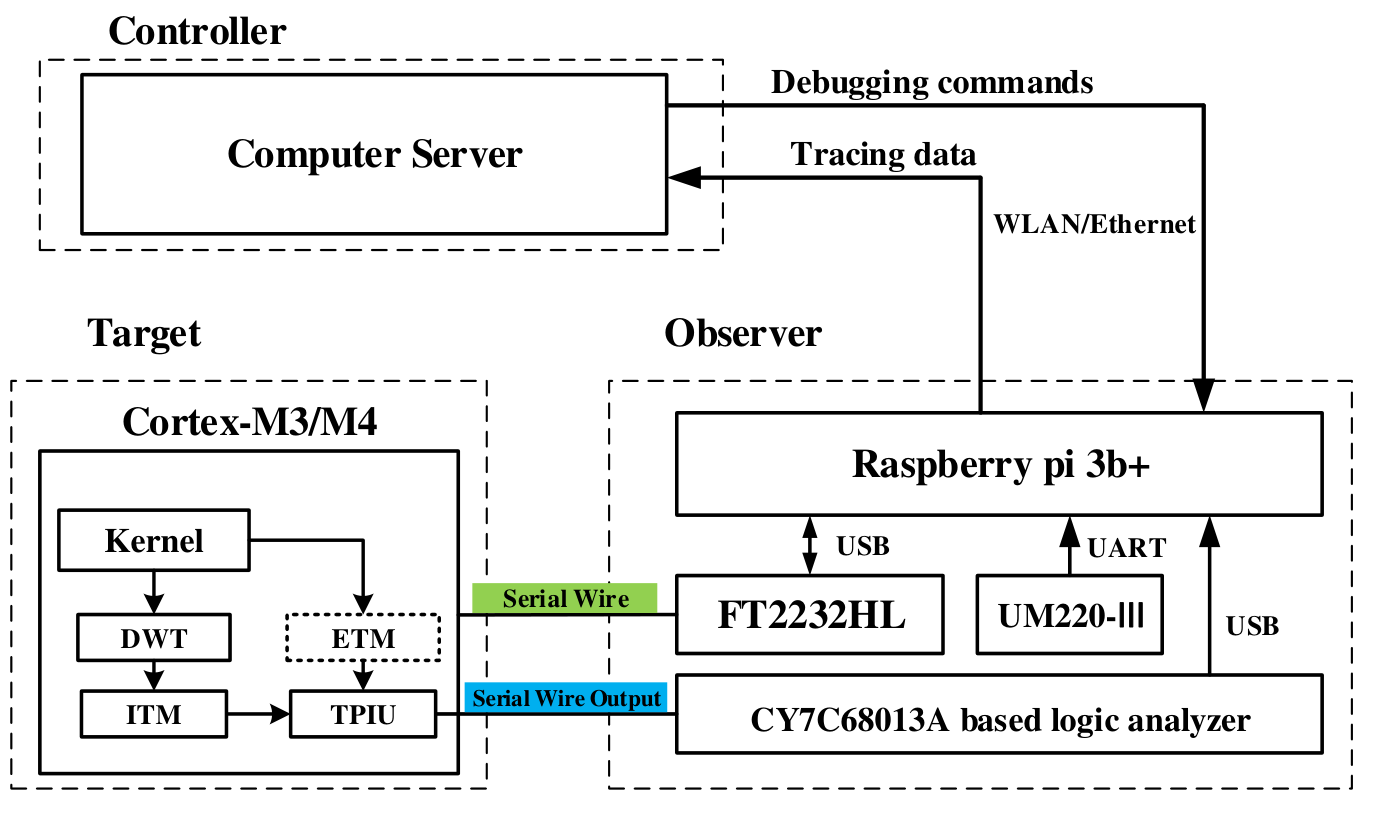
\includegraphics[width=0.80\columnwidth]{hatbed.png}
        \caption{HATBED Architecture}
        \label{fig:bedofnails}
    \end{figure}
\end{frame}

\begin{frame}
  \centering \Large
  \emph{Thank You For Your Attention}
\end{frame}

\begin{frame}[allowframebreaks]
    \frametitle{References}
    \printbibliography
\end{frame}

\begin{frame}
    \frametitle{Calculating Required Bandwidth For Trace Capture}
    \begin{itemize}
        \item IPS: Instruction Per Second (Clock * IPC).
        \item BTL: Branch Token Length in bytes.
        \item IPB: Instruction Per Branch in bytes.
        \item ITMB: ITM Bandwidth in bytes.
        \item TSC: number of trace source changes per 16 bytes of output trace. \cite{arm2020tpiu}
    \end{itemize}
    \begin{equation}
        (\sum_{all cores}(IPS * BTL
        / IPB)) + ITMB) * 16 / (15 - TSC)
    \end{equation}
\end{frame}

\end{document}
